\documentclass{beamer}
\title{Auth Application Refactoring, Stage 2}
\author{Ilya Averyanov}
\institute{EMQX}
\date{2023}
\usetheme{emqx}
\usepackage{listings}
\usepackage{color}
\usepackage{graphicx}
\usepackage{xcolor}
\usepackage{hyperref}
\definecolor{href}{rgb}{0,0,0.9375}
\hypersetup{
    pdfborderstyle={/S/U/W 1}, % underline links instead of boxes
    colorlinks=true,
    urlcolor=href
}
\lstset{frame=tb,
  aboveskip=3mm,
  belowskip=3mm,
  showstringspaces=false,
  columns=flexible,
  basicstyle={\small\ttfamily},
  numbers=none,
  numberstyle=\tiny\color{gray},
  keywordstyle=\color{blue},
  commentstyle=\color{dkgreen},
  stringstyle=\color{mauve},
  breaklines=true,
  breakatwhitespace=false,
  tabsize=2
}


\begin{document}

\frame{\titlepage}

\begin{frame}
    \frametitle{Current State}
    \begin{center}
        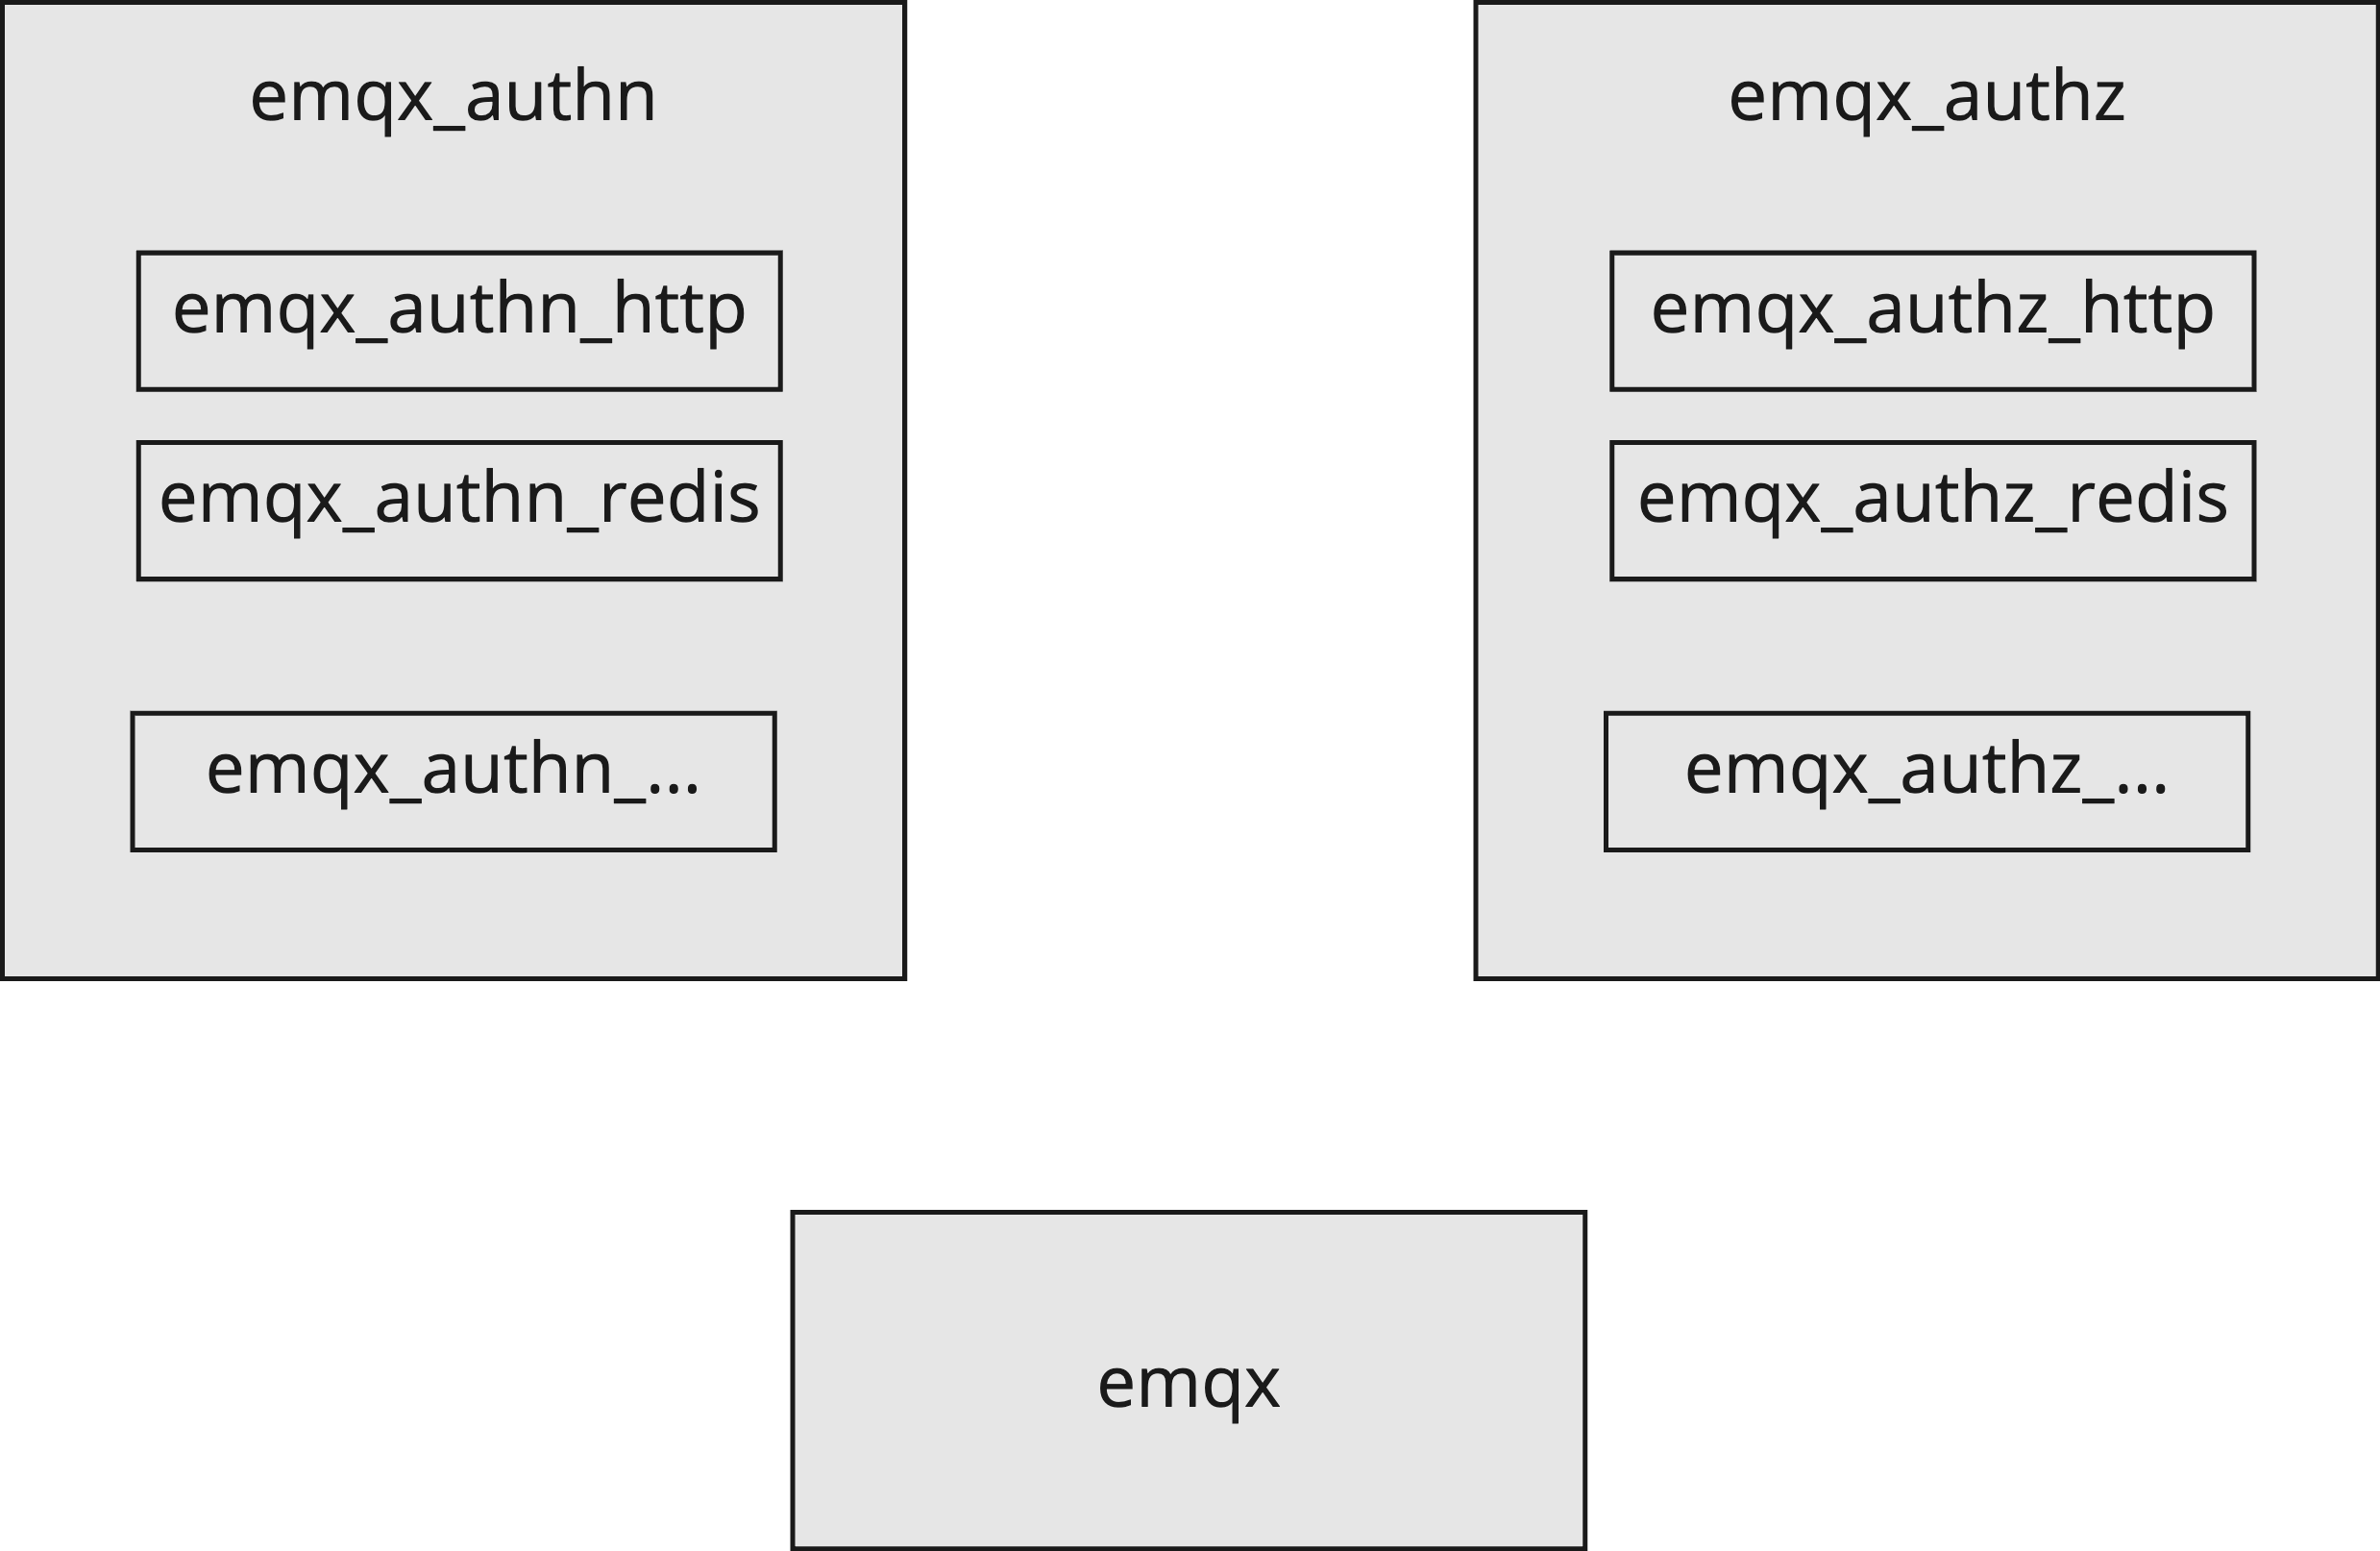
\includegraphics[width=10cm, keepaspectratio]{images/current.png}
    \end{center}
\end{frame}


\begin{frame}
    \frametitle{Desired State}
    \begin{center}
        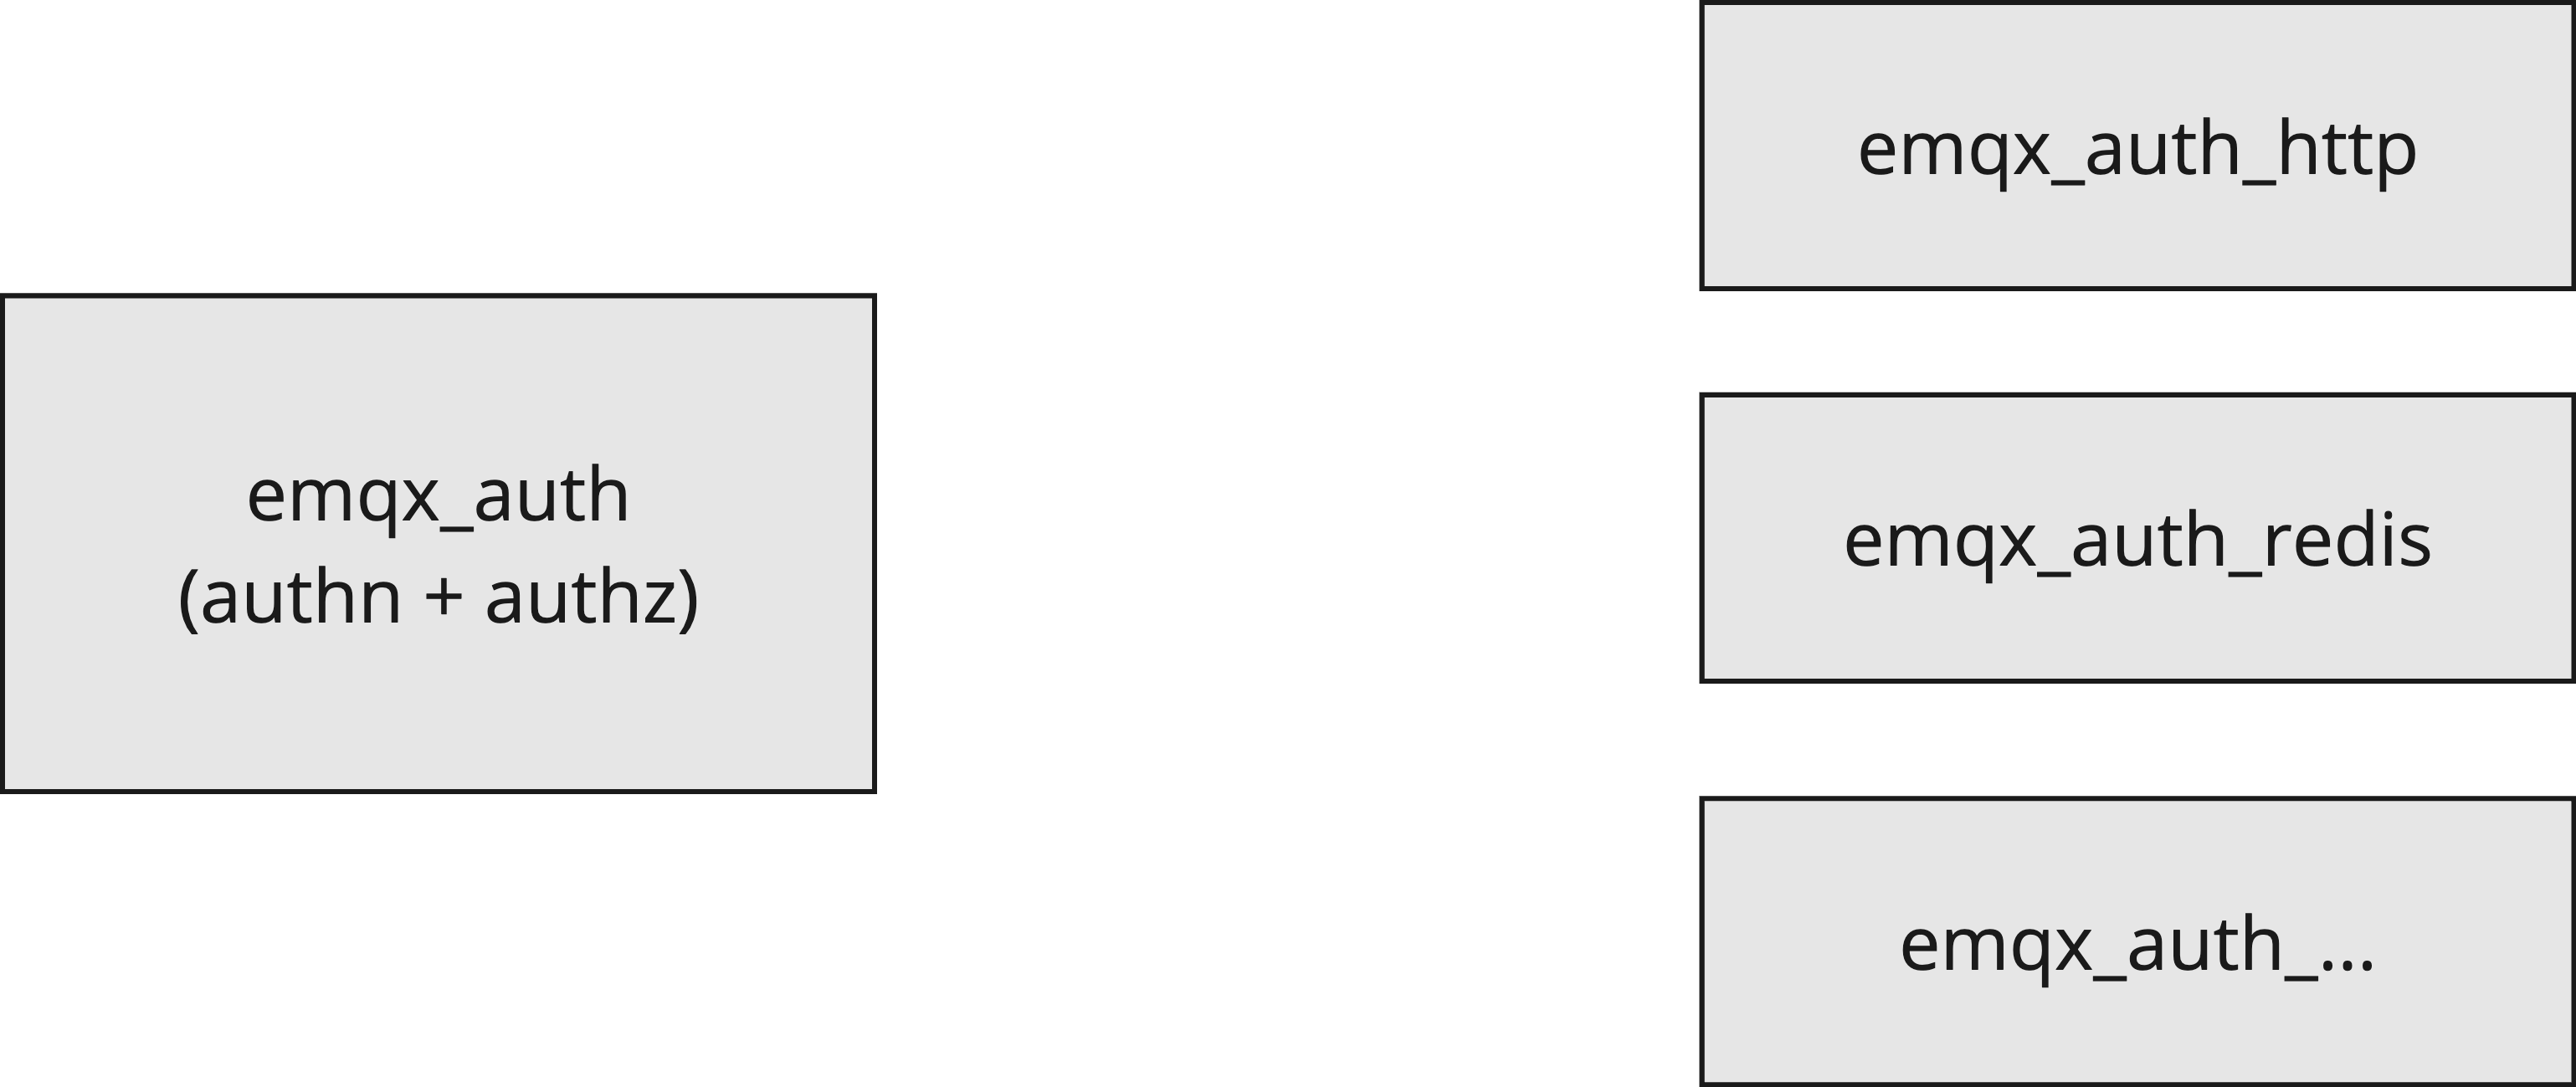
\includegraphics[width=10cm, keepaspectratio]{images/desired.png}
    \end{center}
\end{frame}

\begin{frame}
    \frametitle{Auth Refactoring}
    \framesubtitle{Purposes}

    \begin{center}
        \begin{itemize}
            \item Better separation of concerns
            \item Better application infrastructure (less dependencies, easier hot code reloading, less cumbersome CI)
            \item Better extensibility and pluggability
        \end{itemize}
    \end{center}
\end{frame}


\begin{frame}
    \frametitle{Auth Refactoring}
    \framesubtitle{Naive}

    \begin{center}
        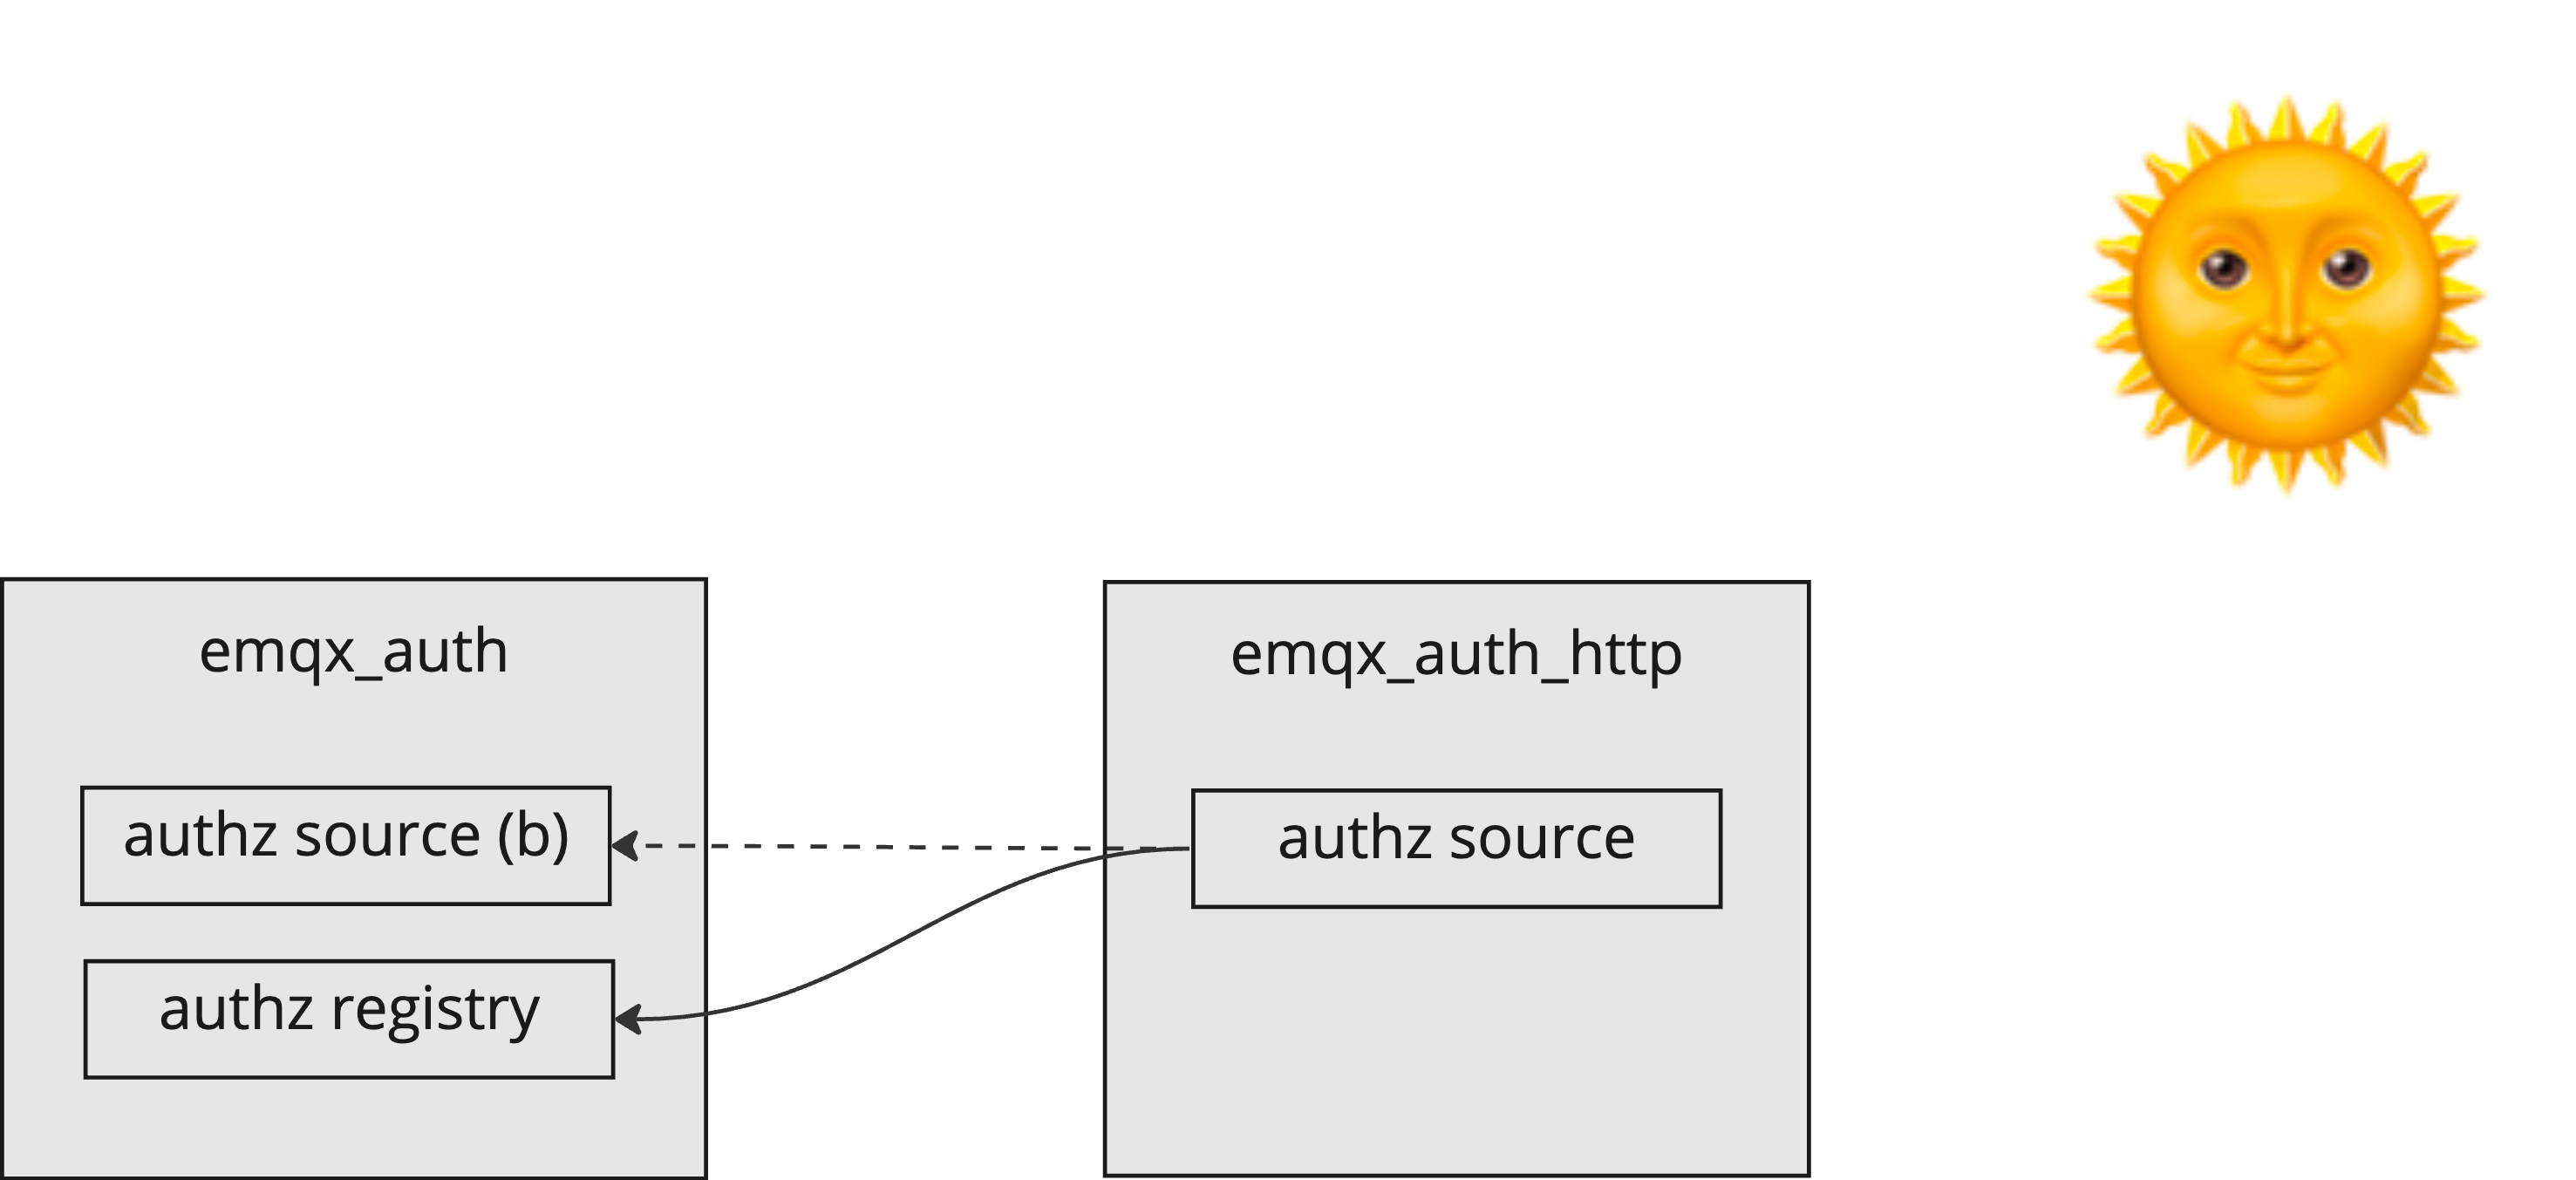
\includegraphics[width=10cm, keepaspectratio]{images/refactor-naive.png}
    \end{center}
\end{frame}


\begin{frame}
    \frametitle{Auth Refactoring}
    \framesubtitle{Actual}

    \begin{center}
        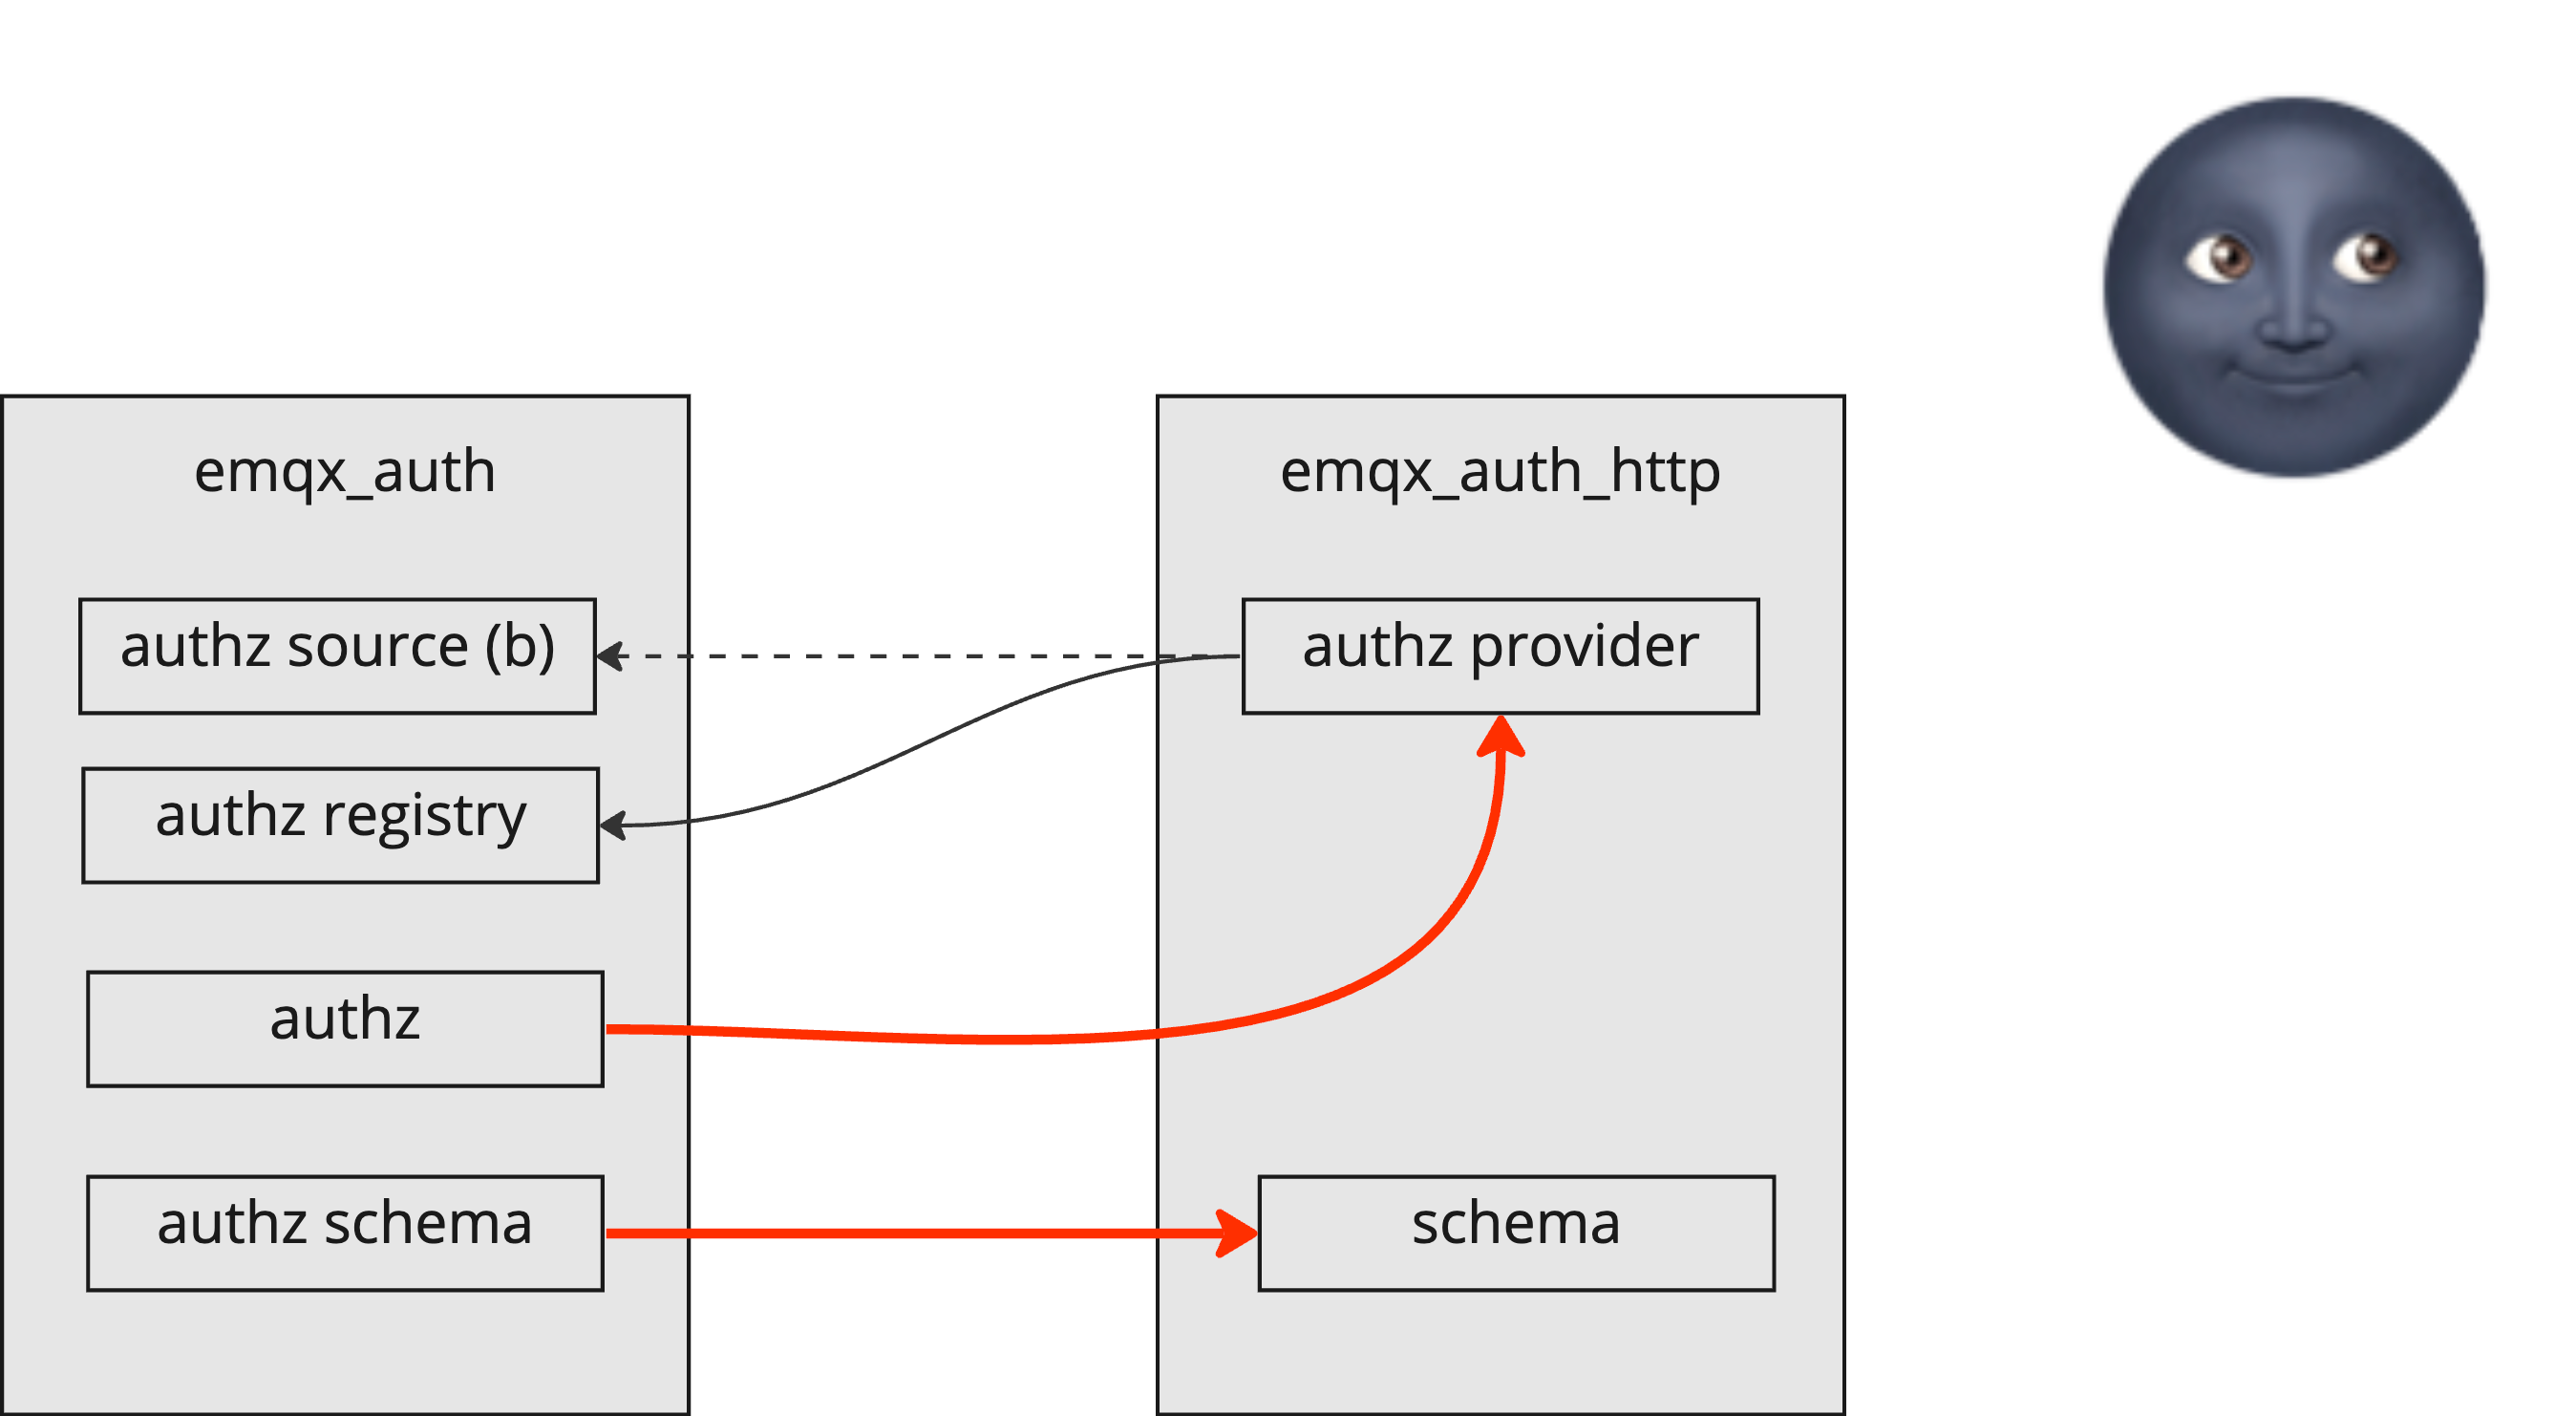
\includegraphics[width=10cm, keepaspectratio]{images/refactor-real.png}
    \end{center}
\end{frame}


\begin{frame}
    \frametitle{Auth Refactoring}
    \framesubtitle{Challenges}

    \begin{center}
        \begin{itemize}
            \item Leaking (ad hoc) transformations of authn provider/authz source data
            \item Opposite directions of dependencies in schema layer and in provider/source layer
            \item Delayed initialization
            \item Lack of top level "profile" IoC container
        \end{itemize}
    \end{center}
\end{frame}


\begin{frame}[fragile]
    \frametitle{Auth Refactoring}
    \framesubtitle{Ad Hoc Transformations}

    \begin{center}
        We extend authn/authz behaviours to make transformations opaque
        \begin{lstlisting}
            %% Some new authz source callbacks

            -callback write_files(raw_source()) -> raw_source() | no_return().
            -callback read_files(raw_source()) -> raw_source() | no_return().
            -callback merge_defaults(raw_source()) -> raw_source().
        \end{lstlisting}
    \end{center}
\end{frame}


\begin{frame}[fragile]
    \frametitle{Auth Refactoring}
    \framesubtitle{Delayed Initialization}

    \begin{center}
        \begin{itemize}
            \item Authn/authz install forbidding hooks on start.
            \item Authn/authz do not instantiate providers/sources on start if there are any nontrivial ones.
            \item On source/privider registration we check if all configured providers/sources are available.
            \item If yes, we instantiate them and install actual checking hooks.
        \end{itemize}
    \end{center}
\end{frame}

\begin{frame}
    \frametitle{Auth Refactoring}
    \framesubtitle{Circular Dependencies}

    \begin{center}
        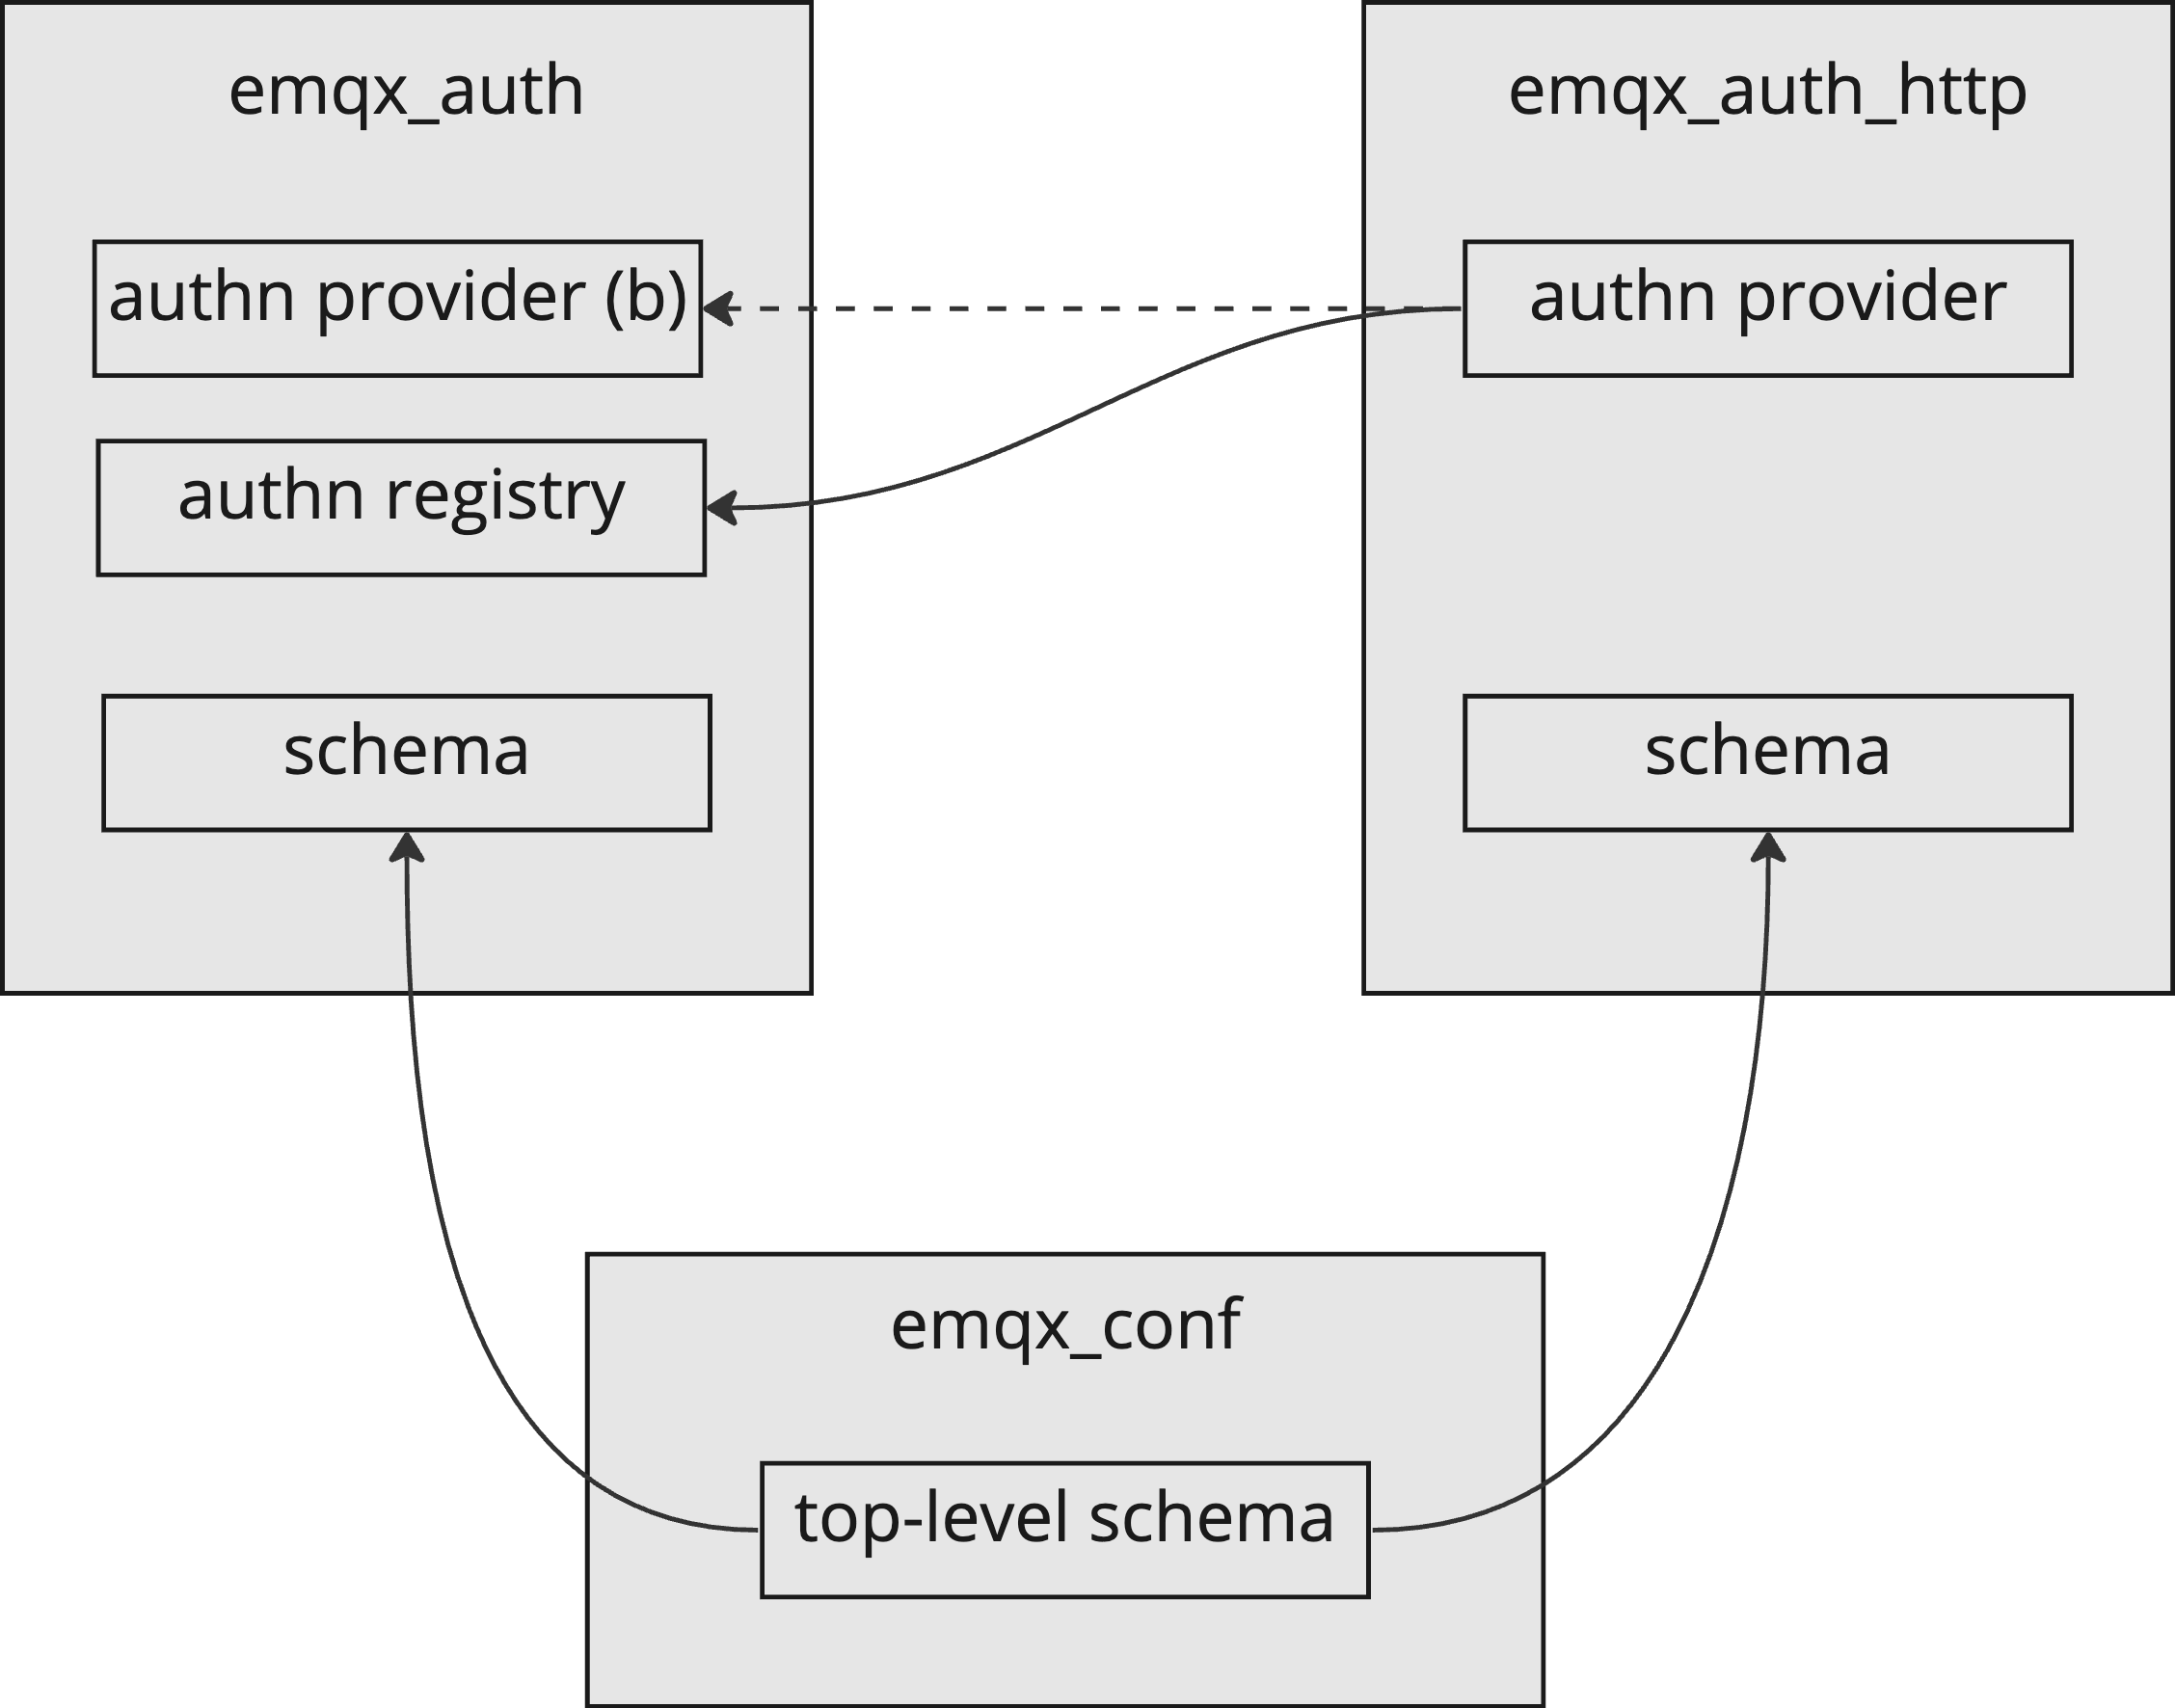
\includegraphics[width=8cm, keepaspectratio]{images/schema-deps.png}
    \end{center}
\end{frame}

\begin{frame}[fragile]
    \frametitle{Auth Refactoring}
    \framesubtitle{Circular Dependencies}

    \begin{center}
        \begin{itemize}
            \item We have inevitable circular dependencies only in schema.
            \item We use \lstinline{emqx_conf} (\lstinline{emqx_conf_schema}) as the plumbing layer (actually, it already is).
            \item \lstinline{emqx_conf} identifies actual provider/source schema modules.
            \item \lstinline{emqx_conf} passes them to the full authn/authz schema modules.
            \item \lstinline{emqx_conf} injects the resulting schema into `emqx` app.
        \end{itemize}
    \end{center}
\end{frame}

\begin{frame}
    \frametitle{Auth Refactoring}
    \framesubtitle{Custom Auth: With Schema Validation}

    \begin{center}
        \begin{itemize}
            \item Implement an application that implements auth and auth schema behaviours, similar to the existing apps.
            \item Also integrate this into the build configs (\lstinline{reboot_lists.eterm}, \lstinline{mix.exs}, etc.).
        \end{itemize}
    \end{center}
\end{frame}

\begin{frame}
    \frametitle{Auth Refactoring}
    \framesubtitle{Custom Auth: With Loose Schema Validation}

    \begin{center}
        \begin{itemize}
            \item \textbf{We} implement generic schema behaviours, which allows to provide an arbitrary option map as (a part of) config (TBD).
            \item \textbf{Customer} implements a full application or just a \textbf{plugin} that implements only source/provider behaviours.
        \end{itemize}
    \end{center}
\end{frame}

\begin{frame}
    \frametitle{Auth Refactoring}
    \framesubtitle{Missing features}
    \begin{center}
        \begin{itemize}
            \item Further \textbf{local} unifications — they are intentionally left for later in order
             not to make the PR too big and containing mixed logic.
            \item Improving READMEs, this is also can be done continously.
        \end{itemize}
    \end{center}
\end{frame}

\begin{frame}
    \begin{center}
        Thank you!
    \end{center}
\end{frame}

\end{document}
